\documentclass{article}
\usepackage{ctex}
\title{编译原理 作业6}
\author{} 
\date{}
\usepackage[a4paper,left=10mm,right=10mm,top=15mm,bottom=15mm]{geometry} 
\usepackage{graphicx} 
\usepackage{makecell}
\usepackage[linguistics]{forest}
\usepackage{amsmath}

\begin{document}

\section*{6.2}
\noindent

\textbf{(1)}
\begin{figure}[htbp]
\centering
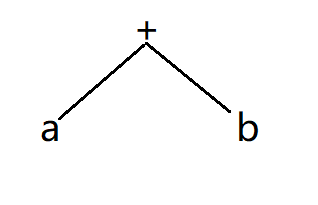
\includegraphics[scale=0.7]{5_1.png}
\end{figure} 

\textbf{(2)}
\begin{figure}[htbp]
\centering
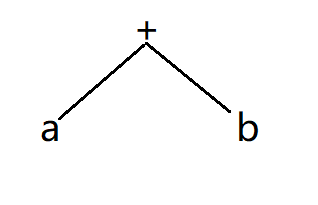
\includegraphics[scale=0.7]{5_1.png}
\end{figure} 

\section*{6.5}
\noindent

\textbf{(1)}
\begin{align*}
    E\rightarrow E_1+T\ \ \ \ &\{if(E_1.type=int)\ and\ (T.type=int)\\
&then\ E.type\ :=\ int\\
&else\ E.type\ :=\ real\}\\
E\rightarrow T\ \ \ \ \ \ \ \ \ \ \ \ &\{E.type\ :=\ T.type\}\\
T\rightarrow num.num&\{T.type\ :=\ real\}\\
T\rightarrow num\ \ \ \ \ \ \ \ &\{T.type\ :=\ int\}
\end{align*}

\section*{7}
\noindent

\begin{align*}
S\rightarrow L_1|L_2&\{S.val\ :=\ L_1.val+(L_2.val/2^{L_2.length})\}\\
S\rightarrow L\ \ \ \ \ \ &\{S.val\ :=\ L.val\}\\
L\rightarrow L_1B\ \ &\{L.val\ :=\ 2*L_1.val+B.val;\\
&L.length\ :=\ L_1.length+1\}\\
L\rightarrow B\ \ \ \ \ \ &\{L.val\ :=\ B.c;\\
&L.length\ :=\ 1\}\\
B\rightarrow 0\ \ \ \ \ \ \ &\{B.c\ :=\ 0\}\\
B\rightarrow 1\ \ \ \ \ \ \ &\{B.c\ :=\ 1\}
\end{align*}

\end{document}